\section{Kociemba's Optimal Solver}
In the following the Kociemba optimal solver\cite{kociemba09} will be described in detiail. Kociemba's Algorithm finds a solution to a scrambled \rubik{} using two phases and is based on another algorithm by Kociemba called Two Phase Algorithm. In order to fully understand kociemba's algorithm a process called relabeling must be defined at first. 

\subsection{Relabeling}
The relabeling process  starts with choosing an up face with a corresponding down face. Then choosing a front face with a corresponding back face. Each \facelet{} with the color of the up or down face is marked with the letters ``UD''.  Each edge \piece{} on the front and back where the \piece{} does not contain a ``UD'' sticker is marked with the letters ``FB''. Figure \ref{fig:relabelClean} shows an example.


\begin{figure}[hb]
	\centering
		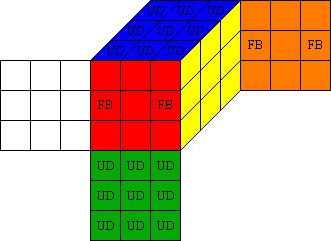
\includegraphics[scale = 0.8]{input/pics/relabelClean}
	\caption{\myCaption{A relabeled Rubik's Cube with the up and down faces blue and green respectively, and red and orange as front and back.}}
	\label{fig:relabelClean}
\end{figure}

When relabeling a \rubik{} in the position $s$ it is written as: $r(s)$. A \rubik{} in any position, $s$, is said to be en the set of positions called $H$ if and only if: $r(s)=r(e)$.

The following moves are in the set of moves $A$: U, U', U2, D, D', D2, R2, L2, F2 and B2. If using move sequences in $A$ on a position in $H$, the cube will always be in $H$. The reason for this can easily be tested with a \rubik{}. If using one of the three up face moves or one of the three down face moves, the ``FB'' labels are not moved and the ``UD'' labels are simply rotated on the face that is being twisted, see figure \ref{fig:relabel2:D}. The last four moves are all very similar to each other. If any side face -- not up or down -- is twisted 180 degrees, the three \facelet{}s on the up face is moved to the down face and vice versa and thereby keeping all the ``UD'' labels on the up and down face and keeping the orientation correct. The two remaining relabeled \facelet{}s are swapped which keeps the ``FB'' labels placed and oriented correctly, see figure \ref{fig:relabel2:R2}.

\begin{figure}[htb]
	\centering
	\subfloat[\myCaption{A relabeled cube that has been permutated with the move D.}]{\label{fig:relabel2:D}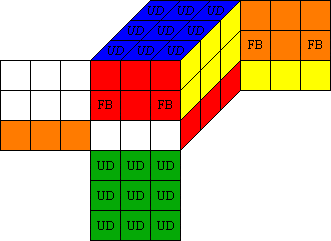
\includegraphics[width=0.45\textwidth]{input/pics/relabelD.PNG}}
	\vspace{0.1\textwidth}
	\subfloat[\myCaption{A relabeled cube that has been permutated with the move R2.}]{\label{fig:relabel2:R2}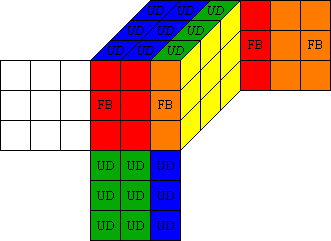
\includegraphics[width=0.45\textwidth]{input/pics/relabelR2.PNG}}
	\caption{\myCaption{Two positions which have been permuted with a move in $A$.}}
	\label{fig:relabel2}
\end{figure}


If using moves in $A$ on a position outside $H$, the cube can not enter $H$.

\subsection{Overall description}
\label{sub:overallDescription}
The first phase takes a scrambled cube $a$ and relabels it $r(a)$ then it finds a move sequence $b$ which will transform the relabeled cube into the subgroup $H$. This move will be denoted: $r(a)\cdot{}b \in H$. The second phase will the determine the length from the position $ab$ to the unit position $e$ by a table lookup. 


\begin{algorithm}                     
\caption{Kociemba's Algorithm \cite{rokicki09}}          
\label{alg:kociemba}        
\begin{algorithmic}[1]
\STATE $d=0$
\STATE {$l=\infty$}
\WHILE {$d<l$} 
	\FOR {$b \in S^{d}$}
		\IF {$r(ab) \in H$}
			\IF {$d + d_{2}(ab)<l$}
				\STATE {$l=d+d_{2}(ab)$}
			\ENDIF
		\ENDIF
	\ENDFOR
	\STATE {$d=d+1$}
\ENDWHILE
\end{algorithmic}
\end{algorithm}

At first in the algorithm the diameter length ($d$), pictured in figure(somewhere) is set to zero and the length($l$) is set to infinite. The \textbf{while} loop will run as long as $d$ is smaller than $l$. For the first run this is true, and will only test if the scrambled cube already is in the subgroup $H$. (If so it will actually continue since a solution that goes out of $H$ might be a faster solution). 

\begin{figure}[hb]
	\centering
		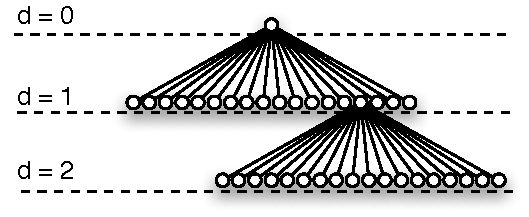
\includegraphics{input/pics/searchExpansion.pdf}
	\caption{\myCaption{As the diameter of the search $d$ increases, the increasing of possible move sequences expands rapidly. For each vertex on the graph there is 18 child vertex. The amount of leaves for each search depth would be $18^{d}$. Note: symmetry is not in considered in this example. }}
	\label{fig:searchExpansion}
\end{figure}

The \textbf{for} loop runs through all move sequences in range $d$ -- recall that $S^d$ is the set containing every move sequence that uses $d$ twists in figure \ref{fig:searchExpansion} it is shown the amount of elements in $S^d$ to a specific $d$. Then an \textbf{if}-statement checks whether the move sequence transforms the cube into the subgroup $H$. If so the algorithm checks whether $d + d_2$ is lesser than the length of the last solution, if so, $d + d_2$ is the new shortest move sequence, $l$, to $e$. $d_2$ is a lookup table which takes a position in $H$ and returns the number of twists it takes to move the position to $e$ using moves in $A$ -- this is further described in the subsection \ref{sub:secondPhase}. The first time this \textbf{if} statement is run it will return true and this will be the new length of the solution. Thereby the \textbf{while} loop will end when $d$ is incremented to $l$.
\begin{figure}[htb]
	\centering
		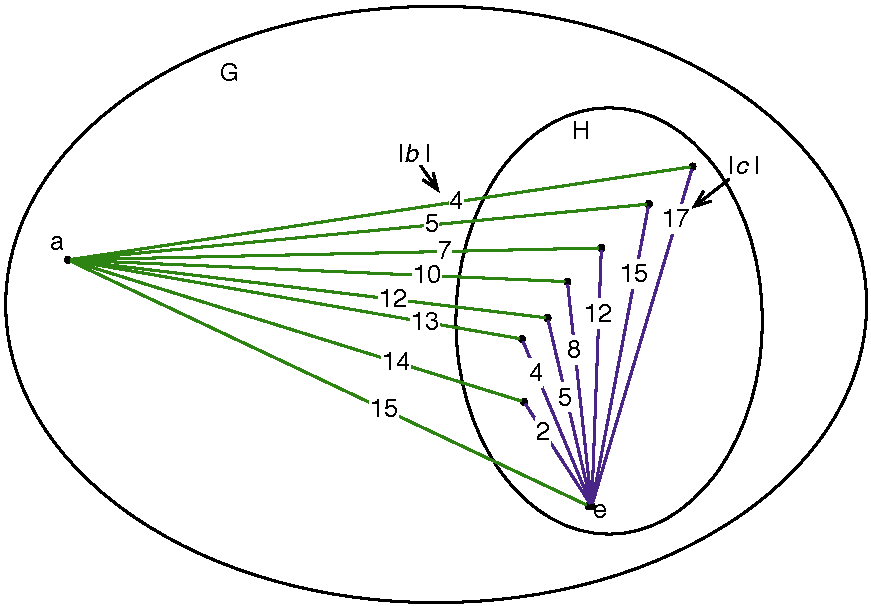
\includegraphics[scale=0.75]{input/pics/kocieambe2.pdf}
	\caption{\myCaption{Here the move sequences the leads to a shorter length in the algorithm is denoted. The lines going from $a$ to a point in $H$ is the move sequence denoted $b$. The lines from points in $H$ to the point $e$ is the move sequence denoted $c$ . The numbers beside the lines are the number of moves. Note that the moves in $c$ is decreasing as the numbers of moves in $b$ is increasing.  }}
	\label{fig:kocieambe2}
\end{figure}

\subsection{First phase}
\label{sub:firstPhase}
...The first phase finds a move sequence, $b$,  from a position $a$ that transform the cube into the subgroup $H$.


\subsection{Second Phase}
\label{sub:secondPhase}
The goal of the second phase is to find the length of the shortest move sequence to transform the cube from a position in $H$ into $e$. The time wise most efficient way to do this is to have a lookup table which has a length for each position in $H$. This table has to be very large, considering the amount of different positions the \rubik{} can be in and still be in $H$. The number of elements in $H$ can be found by multiplying the different positions the different pieces can have. Note that every pieces' orientation must be fixed.


